% !TEX root = ../../技术文档.tex
\section{图像采集与显示链路}

图像采集与显示链路连接外部视频源、DDR3存储器和系统计算模块，完成视频接收、输入预处理、帧缓存读写及显示合成，整体结构如图\ref{fig:video-subsystem}所示。
MS7200将HDMI输入转换为并行RGB888像素，FPGA从同一源帧生成原图和模型输入两类数据并写入DDR；
显示端按行读取已提交的原图，根据模式绘制同帧检测框或合成透明头像，经MS7210输出800$\times$600全屏画面。

像素处理和数据搬运由Video硬件及DMA完成，CPU负责帧调度、检测后处理和显示提交，NPU从输入槽读取张量并执行模型计算图。
应用提供RAW、BOX和AVATAR三种模式，分别显示原图、检测框和透明头像；原图引用、检测及头像参数在有效图像边界整体切换。
每个采集帧写入1,440,000\,B原图和307,200\,B模型输入，共1,747,200\,B。

\begin{figure}[!htbp]
\centering
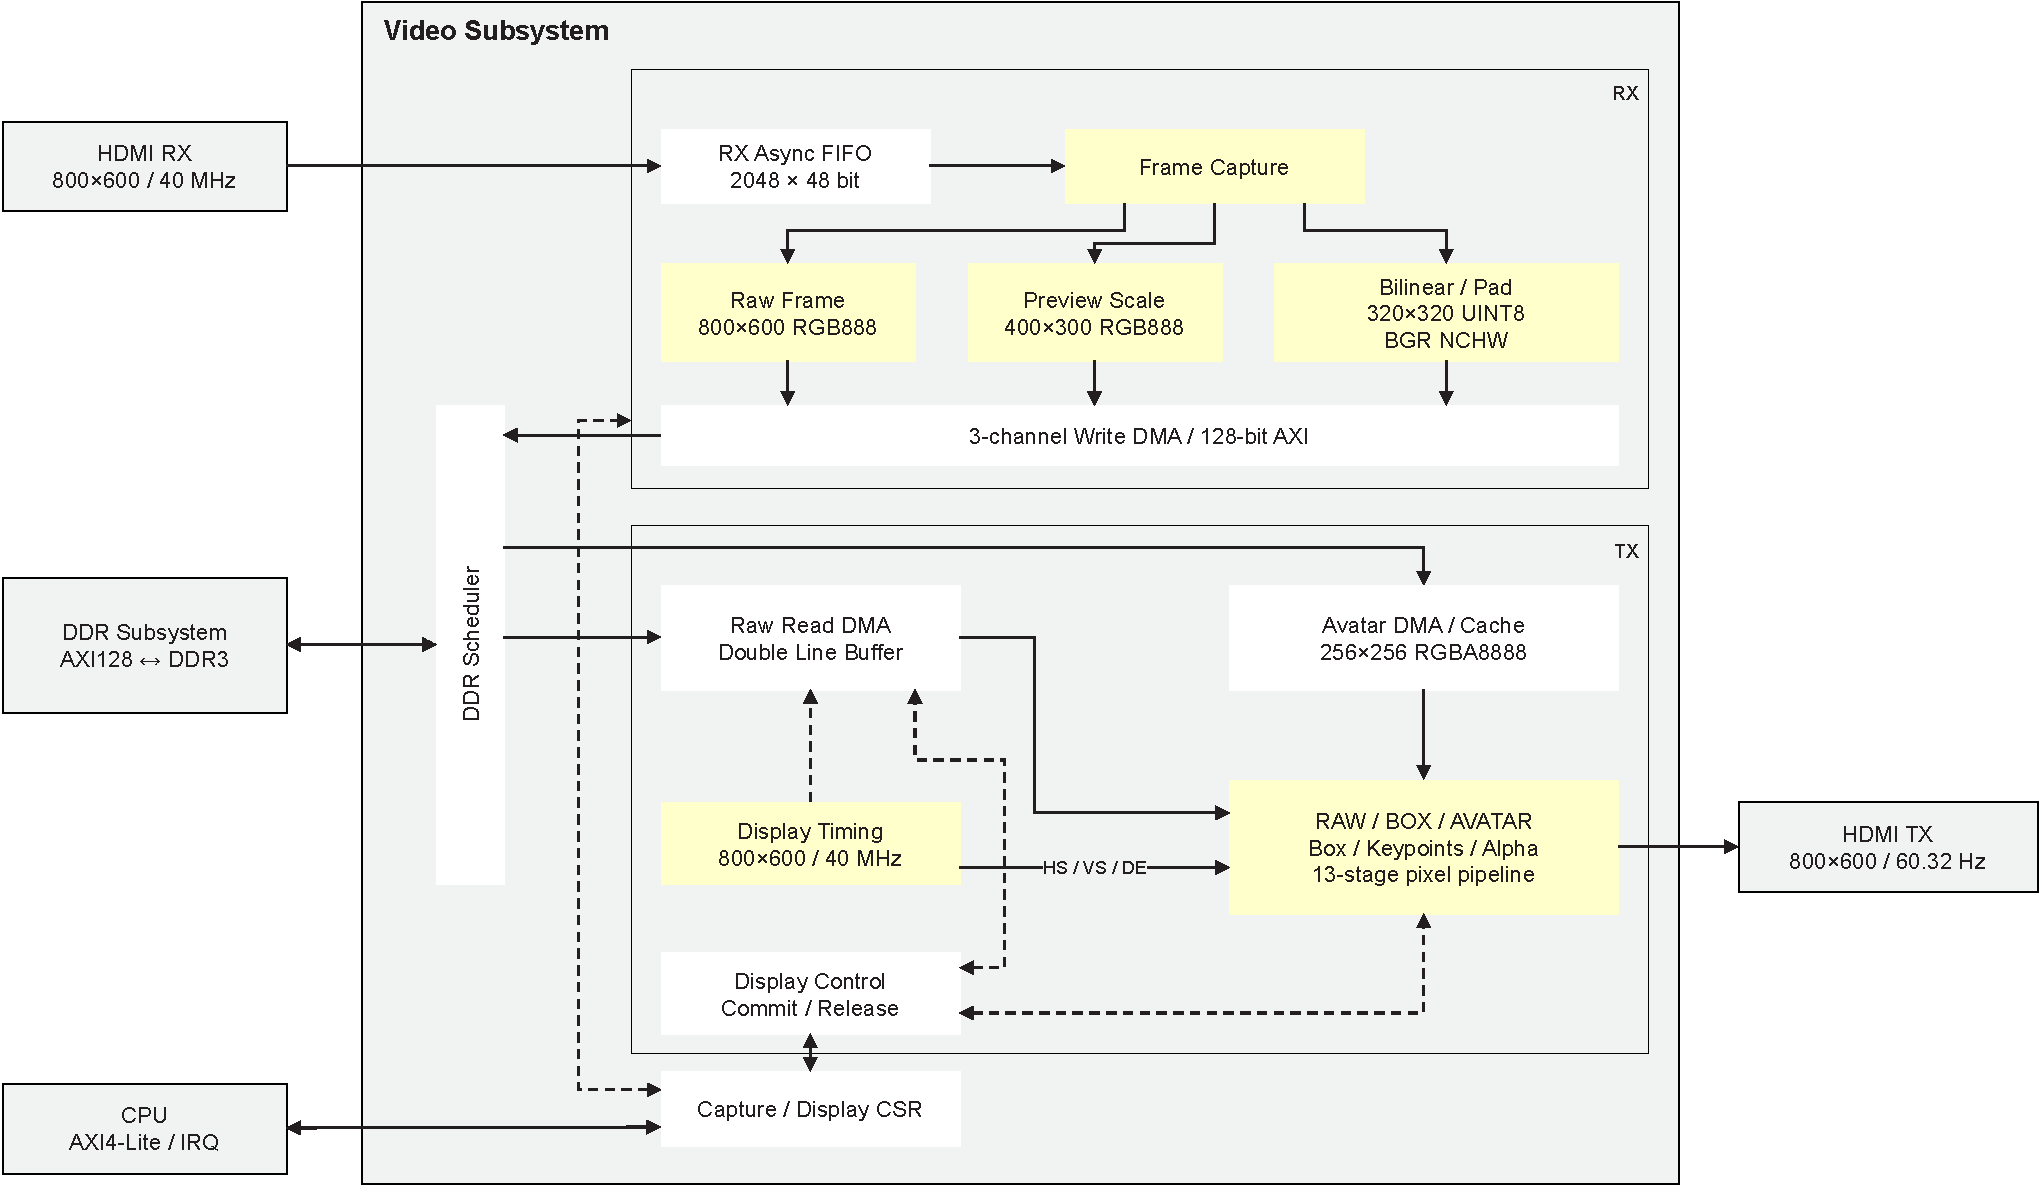
\includegraphics[width=\linewidth]{../figure/rv32-soc-page8.pdf}
\caption{视频子系统结构框图}\label{fig:video-subsystem}
\end{figure}

\subsection{图像采集}

HDMI接收端提供24\,bit RGB888像素，以及输入像素时钟、行同步HS、场同步VS和数据有效DE信号。
HS、VS用于识别行场边界，DE限定有效图像区；消隐期间的数据不写入图像缓冲区。
板级I\textsuperscript{2}C控制器先配置MS7210发送端，再配置MS7200接收端。
时钟锁定和芯片初始化完成后，入口继续检查输入光栅，并经过默认128个连续有效帧的预热过程；
DDR初始化、时钟和接口状态满足要求且模型及素材装载封存后，CPU进入应用循环并提交采集任务。输入与采集参数见表\ref{tbl:video-capture-parameters}。

\begin{reporttable}
\begin{longtable}{@{}p{0.23\linewidth}p{0.29\linewidth}p{0.41\linewidth}@{}}
\caption{视频输入与采集参数}\label{tbl:video-capture-parameters}\\
\toprule
项目 & 配置 & 功能 \\
\midrule
\endfirsthead
\caption[]{视频输入与采集参数（续）}\\
\toprule
项目 & 配置 & 功能 \\
\midrule
\endhead
\bottomrule
\endfoot
输入有效区 & 800$\times$600 & 每帧480000个有效像素 \\
像素格式 & RGB888，24\,bit & 三个颜色分量均为8\,bit无符号数 \\
输入像素时钟 & 标称40\,MHz & 接收随源输入的像素与同步信号 \\
核心处理时钟 & 125\,MHz & 预处理、DMA与存储访问控制 \\
边界与有效信号 & HS、VS、DE & 行场边界及有效区标记 \\
入口跨域缓冲 & 2048项，48\,bit/项 & 像素、行尾及帧结束信息成包传递 \\
完整帧条件 & 几何、计数及校验正确 & 与两路DMA写响应及端口排空状态共同判定完成 \\
\end{longtable}
\end{reporttable}

采集请求锁存槽号、帧号及预处理版本，入口等待下一完整有效帧的起点，再接收该帧。
像素包携带RGB数据和行尾标记，帧结束包携带有效性、CRC及入口缓冲占用信息。
核心域独立核对行尾位置、帧尾状态和原图CRC，并分别统计原图480000个像素和模型有效图像区76800个像素。
完整帧检查、两路DMA写入结果和端口排空条件全部满足后才发布成功完成事件，完成记录同时给出任务标识、有效字节数及预处理版本。

接收像素域与核心域通过异步FIFO连接。核心域仅在原图和模型输入两条路径均可接收当前像素时共同推进，保持两类输出来自同一源帧。
HDMI源按外部像素时钟连续发送，FIFO用于吸收有限速率波动；入口溢出、尺寸或同步异常、CRC错误、DMA故障及DDR就绪丢失均锁存首次检测到的错误原因。
发生故障后停止发布有效完成结果，已接纳的存储事务继续排空；CPU记录错误并停止提交后续任务，保留帧池状态和相关所有权。

\subsection{输入预处理}

原图分支保持800$\times$600和RGB888格式，用于全屏显示；
模型分支生成320$\times$320 UINT8 BGR NCHW张量。两条路径共享帧标识，分别组织输出和DMA写入事务。

模型分支将800$\times$600图像按横纵均为$2/5$的比例缩小为320$\times$240，再在顶部和底部各补40行零值，保持有效图像的4:3宽高比。
固定5:2双线性结构以五个源位置为一组生成两个目标位置，水平和垂直方向交替使用1:3及3:1的权重。
行缓存保存水平加权和，再完成垂直组合；分级截断和最终舍入顺序与整数参考一致。
补边在写入路径中显式生成，每次任务均写入全部补零区域。

输入张量形状为$[1,3,320,320]$，内存按B、G、R三个平面顺序存放，数据类型为UINT8，尺度为1，零点为0。
Video保留0至255的像素数值，模型内部的量化及算子重定标由模型包定义。
每个平面包含102400\,B，每帧共307200\,B；行跨度为320\,B，平面跨度为102400\,B。
像素坐标为$(x,y)$、通道编号为$c$时，输入槽内字节偏移为
\[
\Delta A=c\times102400+y\times320+x,\qquad c\in\{0,1,2\}
\]
其中$c=0,1,2$分别对应B、G、R，$0\leq x,y<320$。
原图按交错RGB字节打包，模型输入按通道平面和行组织，两路写DMA经128\,bit接口和轮转仲裁器共享存储写端口。
CPU核对完成事件中的帧标识、字节数和预处理版本，并按共享存储访问约定确认可见性，再发布输入就绪并启动NPU。

\subsection{帧缓存管理}

帧缓存放置在DDR3，片上保留跨域FIFO、缩放行缓存和显示行缓冲。
公共配置分配三个2\,MiB帧槽和三个320\,KiB模型输入槽；每个帧槽保存原图，同槽号的独立输入槽保存模型张量。
有效数据量与预留容量分开管理，两类数据的组织见表\ref{tbl:video-frame-layout}。

\begin{reporttable}
\begin{longtable}{@{}p{0.15\linewidth}p{0.26\linewidth}p{0.18\linewidth}>{\raggedright\arraybackslash}p{0.34\linewidth}@{}}
\caption{图像数据与缓存组织}\label{tbl:video-frame-layout}\\
\toprule
数据对象 & 尺寸与格式 & 有效数据量 & 槽内布局 \\
\midrule
\endfirsthead
\caption[]{图像数据与缓存组织（续）}\\
\toprule
数据对象 & 尺寸与格式 & 有效数据量 & 槽内布局 \\
\midrule
\endhead
\bottomrule
\endfoot
原图 & 800$\times$600 RGB888 & 1,440,000\,B & 帧槽偏移0，行跨度2400\,B \\
模型输入 & 320$\times$320$\times$3 UINT8 BGR NCHW & 307,200\,B & 独立输入槽，行跨度320\,B \\
固定头像 & 256$\times$256 RGBA8888 & 262,144\,B & 独立素材区，行跨度1024\,B \\
\end{longtable}
\end{reporttable}

Video的采集写入和显示读取分别接入共享DDR互连，与CPU、NPU访问通路共同参与事务轮询。
仲裁器锁存事务来源，保持请求与响应的对应关系，完成当前事务后再选择下一主端。
桥接层完成128\,bit访问与HMIC 256\,bit用户接口之间的转换，行缓冲预取用于衔接存储访问与连续像素输出。

槽号标识物理位置，帧号关联原图、模型输入和结果，代次标识共同复位后的运行会话，槽复用时分配新的帧号；预处理版本限定输入数值含义。
CPU帧池依次维护空闲、采集、就绪、计算、待显示、显示提交等待、正在显示和等待释放状态。
CPU在计算完成记录保持期间读取输出头并完成后处理，构建显示记录后向NPU确认任务完成，再释放整图工作区；显示端独立保持对当前原图和叠加参数的引用。

原图槽在计算、后处理及显示引用期间保持所有权。CPU将同一槽号、帧号和代次的原图引用、检测结果、头像参数及所选模式组成就绪记录，显示记录中的结果帧号与原图帧号一致。
显示端仅在匹配的安全SOF边界将就绪记录整体转为活动记录，首个有效像素实际输出后确认实际提交。在下一份完整记录到达前，HDMI重复扫描当前活动记录，而不追逐最新采集帧。
因此图像内容更新率可以低于扫描刷新率，同帧匹配不要求NPU每个扫描周期均产生新结果。

显示命令接收后进入等待生效状态；首像素反馈返回核心域后，所有权管理模块更新活动记录并发布COMMIT事件。
新帧生效后，旧槽进入等待释放状态，相关读事务完成、行缓冲和像素流水中的引用解除后发布RELEASE事件。
CPU核对提交事件中的槽号、帧号、代次、模式和提交序号，核对释放事件中的槽号、帧号和代次，再通过ACK寄存器确认已处理事件。
释放ACK成功后，硬件和软件帧池才将旧槽恢复为空闲。无空闲槽时，应用等待释放事件后继续分配采集任务。

\subsection{图像叠加}\label{sec:video-overlay}

CPU完成检测框解码、非极大值抑制和原图坐标裁剪后，将最多16个保留框写入显示记录。
主人脸从这些框中按面积最大、分数最高、候选序号最小的顺序确定。
检测框坐标采用800$\times$600原图坐标，左上角包含在矩形内，右下角作为不包含的边界。

RAW模式输出已提交帧的原图，采集、推理和帧调度继续运行。
BOX模式绘制全部有效保留框，边框在矩形内部宽两像素，主人脸框为红色，其余框为绿色。
AVATAR模式在主人脸位置合成固定头像。有效无脸记录撤销框和头像，使三种模式均显示同帧原图。
每个输出像素核对原图槽号、帧号和代次与活动显示记录的一致性，使叠加参数与对应原图共同生效。

头像素材采用256$\times$256 RGBA8888，颜色和透明度均为8位，字节顺序为R、G、B、A，颜色使用非预乘形式。
CPU根据主人脸框的左上角$(x_b,y_b)$、宽$w$、高$h$计算正方形覆盖区域。固定素材的覆盖系数为1.5，锚点为$(128,160)$，其定位过程为
\[
S=\left\lceil\frac{384\max(w,h)}{256}\right\rceil,\qquad
c_x=x_b+\left\lfloor\frac{w}{2}\right\rfloor,\quad
c_y=y_b+\left\lfloor\frac{h}{2}\right\rfloor
\]
\[
x_0=c_x-\left\lfloor\frac{128S}{256}\right\rfloor,\qquad
y_0=c_y-\left\lfloor\frac{160S}{256}\right\rfloor,\qquad
x_1=x_0+S,\quad y_1=y_0+S
\]
目标矩形为$[x_0,x_1)\times[y_0,y_1)$。CPU保留伸出屏幕的矩形部分，显示端只裁剪可见覆盖范围，使画面边缘处的纹理比例保持一致。

Video将覆盖区内像素$(x,y)$映射到素材坐标$(u,v)$，采用向下取整的最近邻采样：
\[
u=\left\lfloor\frac{256(x-x_0)}{S}\right\rfloor,\qquad
v=\left\lfloor\frac{256(y-y_0)}{S}\right\rfloor
\]
坐标映射采用定点流水，每个像素时钟可接收一组坐标。设素材颜色通道为$F$、原图通道为$B$、透明度为$a$，逐通道合成结果为
\[
C=\left\lfloor\frac{aF+(255-a)B+127}{255}\right\rfloor
\]
$a=0$时保持原图，$a=255$时输出素材颜色，中间值按整数规则舍入。输入预处理的5:2双线性缩放与此处的头像最近邻采样分别处理模型输入和显示纹理。

固定头像采用无损行区间缓存。每行保存最左至最右非零RGBA像素之间的完整连续区间，区间外恢复为全零RGBA；区间内部零值及透明像素中的非零RGB数据均保留。
该素材共保存34,331个RGBA字，片上像素载荷为137,324\,B，另设行区间表和控制状态。
装载器封存模型及素材后，头像读取器从DDR读取完整262,144\,B数据并校验CRC，再按行区间写入缓存；最后一次物理写入完成后才发布素材就绪。
缓存身份为素材编号1、代次2，与显示记录共同参与提交校验，运行期间内容保持稳定。
更换固定头像时，素材数据、身份及行区间表配套生成，并重新构建固件和位流。

合成通路以16项、每项84位的环形RAM保存原图颜色、坐标、同步信息及帧号，与纹理读取响应对齐。
上下文写入后第9拍同步读取，第10拍用于混合，原存储项到第16拍才再次写入；复位后的填充计数屏蔽旧内容。
RGB、HS、VS、DE、坐标与帧标识沿像素流水同步传递，合成像素直接送往HDMI发送端，省去整帧叠加图的DDR写回。

\subsection{显示输出}

显示读取器依据已提交记录中的原图地址、行跨度和帧标识按行获取RGB888数据。
每行2400\,B，对应150个128\,bit数据拍；核心域预取下一行，像素域读取当前行，双行缓冲衔接突发访问和连续扫描。
原图和头像读取均采用16\,B对齐、最多16拍的INCR突发，并按剩余数据量及4\,KiB页边界缩短当前事务；读仲裁器锁存来源直至响应完成。
新帧数据准备完成后在有效图像起点切换，准备不足时保留已有有效帧。扫描期间检测供数不足和读响应错误，并锁存故障状态。

输出采用VESA DMT的800$\times$600时序\cite{vesa-dmt-2008}，像素时钟为40\,MHz，光栅参数见表\ref{tbl:video-output-timing}，水平和垂直同步均为正极性。
扫描频率为
\[
f_{\mathrm{scan}}=\frac{40\times10^6}{1056\times628}\approx60.32\,\mathrm{Hz}
\]
扫描频率按重复光栅计数，新图更新率按不同采集帧计数，模型处理率按完成整图推理计数。

\begin{reporttable}
\begin{longtable}{@{}p{0.30\linewidth}p{0.30\linewidth}p{0.30\linewidth}@{}}
\caption{显示光栅时序参数}\label{tbl:video-output-timing}\\
\toprule
时序项目 & 水平方向（像素时钟） & 垂直方向（行） \\
\midrule
\endfirsthead
\caption[]{显示光栅时序参数（续）}\\
\toprule
时序项目 & 水平方向（像素时钟） & 垂直方向（行） \\
\midrule
\endhead
\bottomrule
\endfoot
有效区 & 800 & 600 \\
前肩 & 40 & 1 \\
同步脉宽 & 128 & 4 \\
后肩 & 88 & 23 \\
总周期 & 1056 & 628 \\
同步极性 & 正极性 & 正极性 \\
\end{longtable}
\end{reporttable}

固件初始选择RAW模式，KEY1按RAW、BOX、AVATAR顺序循环请求模式。
CPU通过显示接口写入640\,B记录，填充原图地址、行跨度、槽号、帧号及代次、结果标识、检测框、主框索引、素材身份及头像目标矩形，再写入显示模式、提交序号并发出提交请求。
没有新帧时，CPU可对活动帧进行仅模式更新；硬件逐字核对完整记录，保持原图与检测结果不变。
显示接口以RAM保存完整影子记录及活动历史，内部准备寄存器保留32字头部和16组各2字矩形坐标，另用标志记录非法载荷，外部160字接口保持完整。
硬件检查记录格式、地址范围和帧身份，带头像的非空记录还需等待素材就绪并匹配素材身份；跨域握手期间保持整组参数稳定，在匹配的有效图像起点整体应用。
VSYNC维持固定的扫描光栅，COMMIT反馈标识新记录的实际像素生效；旧帧引用解除后另行返回RELEASE事件。
显示接口分别保持提交和释放事件，供CPU读取并确认。
